% Options for packages loaded elsewhere
\PassOptionsToPackage{unicode}{hyperref}
\PassOptionsToPackage{hyphens}{url}
%
\documentclass[
]{article}
\usepackage{amsmath,amssymb}
\usepackage{lmodern}
\usepackage{iftex}
\ifPDFTeX
  \usepackage[T1]{fontenc}
  \usepackage[utf8]{inputenc}
  \usepackage{textcomp} % provide euro and other symbols
\else % if luatex or xetex
  \usepackage{unicode-math}
  \defaultfontfeatures{Scale=MatchLowercase}
  \defaultfontfeatures[\rmfamily]{Ligatures=TeX,Scale=1}
\fi
% Use upquote if available, for straight quotes in verbatim environments
\IfFileExists{upquote.sty}{\usepackage{upquote}}{}
\IfFileExists{microtype.sty}{% use microtype if available
  \usepackage[]{microtype}
  \UseMicrotypeSet[protrusion]{basicmath} % disable protrusion for tt fonts
}{}
\makeatletter
\@ifundefined{KOMAClassName}{% if non-KOMA class
  \IfFileExists{parskip.sty}{%
    \usepackage{parskip}
  }{% else
    \setlength{\parindent}{0pt}
    \setlength{\parskip}{6pt plus 2pt minus 1pt}}
}{% if KOMA class
  \KOMAoptions{parskip=half}}
\makeatother
\usepackage{xcolor}
\usepackage[margin=1in]{geometry}
\usepackage{color}
\usepackage{fancyvrb}
\newcommand{\VerbBar}{|}
\newcommand{\VERB}{\Verb[commandchars=\\\{\}]}
\DefineVerbatimEnvironment{Highlighting}{Verbatim}{commandchars=\\\{\}}
% Add ',fontsize=\small' for more characters per line
\usepackage{framed}
\definecolor{shadecolor}{RGB}{248,248,248}
\newenvironment{Shaded}{\begin{snugshade}}{\end{snugshade}}
\newcommand{\AlertTok}[1]{\textcolor[rgb]{0.94,0.16,0.16}{#1}}
\newcommand{\AnnotationTok}[1]{\textcolor[rgb]{0.56,0.35,0.01}{\textbf{\textit{#1}}}}
\newcommand{\AttributeTok}[1]{\textcolor[rgb]{0.77,0.63,0.00}{#1}}
\newcommand{\BaseNTok}[1]{\textcolor[rgb]{0.00,0.00,0.81}{#1}}
\newcommand{\BuiltInTok}[1]{#1}
\newcommand{\CharTok}[1]{\textcolor[rgb]{0.31,0.60,0.02}{#1}}
\newcommand{\CommentTok}[1]{\textcolor[rgb]{0.56,0.35,0.01}{\textit{#1}}}
\newcommand{\CommentVarTok}[1]{\textcolor[rgb]{0.56,0.35,0.01}{\textbf{\textit{#1}}}}
\newcommand{\ConstantTok}[1]{\textcolor[rgb]{0.00,0.00,0.00}{#1}}
\newcommand{\ControlFlowTok}[1]{\textcolor[rgb]{0.13,0.29,0.53}{\textbf{#1}}}
\newcommand{\DataTypeTok}[1]{\textcolor[rgb]{0.13,0.29,0.53}{#1}}
\newcommand{\DecValTok}[1]{\textcolor[rgb]{0.00,0.00,0.81}{#1}}
\newcommand{\DocumentationTok}[1]{\textcolor[rgb]{0.56,0.35,0.01}{\textbf{\textit{#1}}}}
\newcommand{\ErrorTok}[1]{\textcolor[rgb]{0.64,0.00,0.00}{\textbf{#1}}}
\newcommand{\ExtensionTok}[1]{#1}
\newcommand{\FloatTok}[1]{\textcolor[rgb]{0.00,0.00,0.81}{#1}}
\newcommand{\FunctionTok}[1]{\textcolor[rgb]{0.00,0.00,0.00}{#1}}
\newcommand{\ImportTok}[1]{#1}
\newcommand{\InformationTok}[1]{\textcolor[rgb]{0.56,0.35,0.01}{\textbf{\textit{#1}}}}
\newcommand{\KeywordTok}[1]{\textcolor[rgb]{0.13,0.29,0.53}{\textbf{#1}}}
\newcommand{\NormalTok}[1]{#1}
\newcommand{\OperatorTok}[1]{\textcolor[rgb]{0.81,0.36,0.00}{\textbf{#1}}}
\newcommand{\OtherTok}[1]{\textcolor[rgb]{0.56,0.35,0.01}{#1}}
\newcommand{\PreprocessorTok}[1]{\textcolor[rgb]{0.56,0.35,0.01}{\textit{#1}}}
\newcommand{\RegionMarkerTok}[1]{#1}
\newcommand{\SpecialCharTok}[1]{\textcolor[rgb]{0.00,0.00,0.00}{#1}}
\newcommand{\SpecialStringTok}[1]{\textcolor[rgb]{0.31,0.60,0.02}{#1}}
\newcommand{\StringTok}[1]{\textcolor[rgb]{0.31,0.60,0.02}{#1}}
\newcommand{\VariableTok}[1]{\textcolor[rgb]{0.00,0.00,0.00}{#1}}
\newcommand{\VerbatimStringTok}[1]{\textcolor[rgb]{0.31,0.60,0.02}{#1}}
\newcommand{\WarningTok}[1]{\textcolor[rgb]{0.56,0.35,0.01}{\textbf{\textit{#1}}}}
\usepackage{graphicx}
\makeatletter
\def\maxwidth{\ifdim\Gin@nat@width>\linewidth\linewidth\else\Gin@nat@width\fi}
\def\maxheight{\ifdim\Gin@nat@height>\textheight\textheight\else\Gin@nat@height\fi}
\makeatother
% Scale images if necessary, so that they will not overflow the page
% margins by default, and it is still possible to overwrite the defaults
% using explicit options in \includegraphics[width, height, ...]{}
\setkeys{Gin}{width=\maxwidth,height=\maxheight,keepaspectratio}
% Set default figure placement to htbp
\makeatletter
\def\fps@figure{htbp}
\makeatother
\setlength{\emergencystretch}{3em} % prevent overfull lines
\providecommand{\tightlist}{%
  \setlength{\itemsep}{0pt}\setlength{\parskip}{0pt}}
\setcounter{secnumdepth}{-\maxdimen} % remove section numbering
\ifLuaTeX
  \usepackage{selnolig}  % disable illegal ligatures
\fi
\IfFileExists{bookmark.sty}{\usepackage{bookmark}}{\usepackage{hyperref}}
\IfFileExists{xurl.sty}{\usepackage{xurl}}{} % add URL line breaks if available
\urlstyle{same} % disable monospaced font for URLs
\hypersetup{
  pdftitle={dung\_beetle\_rarefaction},
  pdfauthor={Chloe Cho},
  hidelinks,
  pdfcreator={LaTeX via pandoc}}

\title{dung\_beetle\_rarefaction}
\author{Chloe Cho}
\date{2023-12-08}

\begin{document}
\maketitle

\hypertarget{read-and-clean-data}{%
\section{Read and Clean Data}\label{read-and-clean-data}}

\begin{Shaded}
\begin{Highlighting}[]
\NormalTok{beetle\_counts }\OtherTok{\textless{}{-}} \FunctionTok{read.delim}\NormalTok{(}\StringTok{"../Data/Dung\_Beetle\_Data.csv"}\NormalTok{, }\AttributeTok{sep =} \StringTok{","}\NormalTok{)}
\NormalTok{beetle\_counts }\OtherTok{\textless{}{-}} \FunctionTok{clean\_names}\NormalTok{(beetle\_counts)}
\FunctionTok{head}\NormalTok{(beetle\_counts)}
\end{Highlighting}
\end{Shaded}

\begin{verbatim}
##      date       farm  region temp  weather non_or_insecticide
## 1 5/18/22 Boone Farm Capital   60 Sunshine        Insecticide
## 2 5/25/22 Boone Farm Capital   66 Sunshine        Insecticide
## 3  6/1/22 Boone Farm Capital   68     Rain        Insecticide
## 4  6/7/22 Boone Farm Capital   71   Cloudy        Insecticide
## 5 6/14/22 Boone Farm Capital   68     Rain        Insecticide
## 6 6/22/22 Boone Farm Capital   56     Rain        Insecticide
##   active_ingredients calamosternus_granarius colobopterus_erraticus
## 1      Diflubenzuron                      NA                     20
## 2      Diflubenzuron                      NA                     NA
## 3      Diflubenzuron                       1                     32
## 4      Diflubenzuron                       1                      1
## 5      Diflubenzuron                       1                      2
## 6      Diflubenzuron                      NA                     NA
##   aphodius_fimetarius_pedellus otophorus_haemorrhoidalis oscarinus_rusicola
## 1                           NA                         2                 NA
## 2                           NA                        NA                 NA
## 3                           NA                         1                 NA
## 4                           NA                        NA                 NA
## 5                           NA                        NA                 NA
## 6                           NA                        NA                 NA
##   alloblackburneus_rubeolus acrossus_rubripennis teuchestes_fossor
## 1                        NA                   NA                NA
## 2                        NA                   NA                NA
## 3                        NA                   NA                NA
## 4                        NA                   NA                NA
## 5                        NA                   NA                NA
## 6                        NA                   NA                 2
##   labarrus_pseudolividus_lividus blackburneus_stercorosus pseudagolius_bicolor
## 1                             NA                       NA                   NA
## 2                             NA                       NA                   NA
## 3                             NA                       NA                   NA
## 4                             NA                        1                   NA
## 5                             NA                        2                   NA
## 6                             NA                       NA                   NA
##   eupleurus_subterraneus onthophagus_taurus onthophagus_pennsylvanicus
## 1                     NA                 NA                         NA
## 2                     NA                 NA                         NA
## 3                     NA                  1                         NA
## 4                     NA                  1                         NA
## 5                     NA                 NA                          5
## 6                     NA                 NA                         NA
##   onthophagus_hecate histeridae hydrophilidae staphylinidae scarabaeidae
## 1                 NA         NA            47             3           22
## 2                 NA         NA             2            NA            0
## 3                 NA          1            59             2           35
## 4                 NA         NA            14            NA            4
## 5                 NA         NA            18            NA           10
## 6                 NA          1             9             2            2
##   horn_flies face_flies                                   gps
## 1          2          0 42.54463393478293, -74.03369647630593
## 2          3          1 42.54463393478293, -74.03369647630593
## 3         NA         NA 42.54463393478293, -74.03369647630593
## 4         17          5 42.54463393478293, -74.03369647630593
## 5         27          9 42.54463393478293, -74.03369647630593
## 6          9          6 42.54463393478293, -74.03369647630593
\end{verbatim}

\begin{Shaded}
\begin{Highlighting}[]
\NormalTok{beetle\_counts }\OtherTok{\textless{}{-}}\NormalTok{ beetle\_counts }\SpecialCharTok{\%\textgreater{}\%}
  \FunctionTok{mutate}\NormalTok{(}\AttributeTok{non\_or\_insecticide =} \FunctionTok{tolower}\NormalTok{(non\_or\_insecticide)) }\SpecialCharTok{\%\textgreater{}\%}
  \FunctionTok{mutate}\NormalTok{(}\AttributeTok{weather =} \FunctionTok{tolower}\NormalTok{(weather)) }\SpecialCharTok{\%\textgreater{}\%}
  \FunctionTok{mutate}\NormalTok{(}\AttributeTok{farm =} \FunctionTok{tolower}\NormalTok{(farm)) }\SpecialCharTok{\%\textgreater{}\%}
  \FunctionTok{mutate}\NormalTok{(}\AttributeTok{active\_ingredients =} \FunctionTok{tolower}\NormalTok{(active\_ingredients)) }\SpecialCharTok{\%\textgreater{}\%}
  \FunctionTok{mutate}\NormalTok{(}\AttributeTok{region =} \FunctionTok{tolower}\NormalTok{(region)) }

\FunctionTok{head}\NormalTok{(beetle\_counts)}
\end{Highlighting}
\end{Shaded}

\begin{verbatim}
##      date       farm  region temp  weather non_or_insecticide
## 1 5/18/22 boone farm capital   60 sunshine        insecticide
## 2 5/25/22 boone farm capital   66 sunshine        insecticide
## 3  6/1/22 boone farm capital   68     rain        insecticide
## 4  6/7/22 boone farm capital   71   cloudy        insecticide
## 5 6/14/22 boone farm capital   68     rain        insecticide
## 6 6/22/22 boone farm capital   56     rain        insecticide
##   active_ingredients calamosternus_granarius colobopterus_erraticus
## 1      diflubenzuron                      NA                     20
## 2      diflubenzuron                      NA                     NA
## 3      diflubenzuron                       1                     32
## 4      diflubenzuron                       1                      1
## 5      diflubenzuron                       1                      2
## 6      diflubenzuron                      NA                     NA
##   aphodius_fimetarius_pedellus otophorus_haemorrhoidalis oscarinus_rusicola
## 1                           NA                         2                 NA
## 2                           NA                        NA                 NA
## 3                           NA                         1                 NA
## 4                           NA                        NA                 NA
## 5                           NA                        NA                 NA
## 6                           NA                        NA                 NA
##   alloblackburneus_rubeolus acrossus_rubripennis teuchestes_fossor
## 1                        NA                   NA                NA
## 2                        NA                   NA                NA
## 3                        NA                   NA                NA
## 4                        NA                   NA                NA
## 5                        NA                   NA                NA
## 6                        NA                   NA                 2
##   labarrus_pseudolividus_lividus blackburneus_stercorosus pseudagolius_bicolor
## 1                             NA                       NA                   NA
## 2                             NA                       NA                   NA
## 3                             NA                       NA                   NA
## 4                             NA                        1                   NA
## 5                             NA                        2                   NA
## 6                             NA                       NA                   NA
##   eupleurus_subterraneus onthophagus_taurus onthophagus_pennsylvanicus
## 1                     NA                 NA                         NA
## 2                     NA                 NA                         NA
## 3                     NA                  1                         NA
## 4                     NA                  1                         NA
## 5                     NA                 NA                          5
## 6                     NA                 NA                         NA
##   onthophagus_hecate histeridae hydrophilidae staphylinidae scarabaeidae
## 1                 NA         NA            47             3           22
## 2                 NA         NA             2            NA            0
## 3                 NA          1            59             2           35
## 4                 NA         NA            14            NA            4
## 5                 NA         NA            18            NA           10
## 6                 NA          1             9             2            2
##   horn_flies face_flies                                   gps
## 1          2          0 42.54463393478293, -74.03369647630593
## 2          3          1 42.54463393478293, -74.03369647630593
## 3         NA         NA 42.54463393478293, -74.03369647630593
## 4         17          5 42.54463393478293, -74.03369647630593
## 5         27          9 42.54463393478293, -74.03369647630593
## 6          9          6 42.54463393478293, -74.03369647630593
\end{verbatim}

\begin{Shaded}
\begin{Highlighting}[]
\NormalTok{beetle\_counts }\OtherTok{\textless{}{-}}\NormalTok{ beetle\_counts }\SpecialCharTok{\%\textgreater{}\%}
  \FunctionTok{mutate}\NormalTok{(}\AttributeTok{farm =} \FunctionTok{as.factor}\NormalTok{(farm)) }\SpecialCharTok{\%\textgreater{}\%}
  \FunctionTok{mutate}\NormalTok{(}\AttributeTok{region =} \FunctionTok{as.factor}\NormalTok{(region)) }\SpecialCharTok{\%\textgreater{}\%}
  \FunctionTok{mutate}\NormalTok{(}\AttributeTok{weather =} \FunctionTok{as.factor}\NormalTok{(weather)) }\SpecialCharTok{\%\textgreater{}\%}
  \FunctionTok{mutate}\NormalTok{(}\AttributeTok{non\_or\_insecticide =} \FunctionTok{as.factor}\NormalTok{(non\_or\_insecticide)) }\SpecialCharTok{\%\textgreater{}\%}
  \FunctionTok{mutate}\NormalTok{(}\AttributeTok{active\_ingredients =} \FunctionTok{as.factor}\NormalTok{(active\_ingredients)) }\SpecialCharTok{\%\textgreater{}\%}
  \FunctionTok{mutate}\NormalTok{(}\AttributeTok{date =} \FunctionTok{as.factor}\NormalTok{(date)) }\SpecialCharTok{\%\textgreater{}\%}
  \FunctionTok{mutate}\NormalTok{(}\AttributeTok{date =} \FunctionTok{as.Date}\NormalTok{(date, }\AttributeTok{format=}\StringTok{"\%m/\%d/\%y"}\NormalTok{))}
\end{Highlighting}
\end{Shaded}

\begin{Shaded}
\begin{Highlighting}[]
\NormalTok{beetle\_counts }\OtherTok{\textless{}{-}}\NormalTok{ beetle\_counts }\SpecialCharTok{\%\textgreater{}\%}
  \FunctionTok{mutate}\NormalTok{(}\AttributeTok{non\_or\_insecticide =} \FunctionTok{case\_when}\NormalTok{(non\_or\_insecticide }\SpecialCharTok{==} \StringTok{\textquotesingle{}non   \textquotesingle{}} \SpecialCharTok{\textasciitilde{}} \StringTok{\textquotesingle{}non\textquotesingle{}}\NormalTok{,}
\NormalTok{                                        non\_or\_insecticide }\SpecialCharTok{==} \StringTok{\textquotesingle{}insecticide\textquotesingle{}} \SpecialCharTok{\textasciitilde{}} \StringTok{\textquotesingle{}insecticide\textquotesingle{}}\NormalTok{,}
\NormalTok{                                        non\_or\_insecticide }\SpecialCharTok{==} \StringTok{\textquotesingle{}non\textquotesingle{}} \SpecialCharTok{\textasciitilde{}} \StringTok{\textquotesingle{}non\textquotesingle{}}\NormalTok{))}

\NormalTok{beetle\_counts }\OtherTok{\textless{}{-}}\NormalTok{ beetle\_counts }\SpecialCharTok{\%\textgreater{}\%}
  \FunctionTok{select}\NormalTok{(}\SpecialCharTok{{-}}\FunctionTok{c}\NormalTok{(date, region, temp, weather, non\_or\_insecticide, active\_ingredients, gps, histeridae, hydrophilidae, staphylinidae, scarabaeidae, horn\_flies, face\_flies)) }\SpecialCharTok{\%\textgreater{}\%}
  \FunctionTok{rename}\NormalTok{(}\AttributeTok{site =}\NormalTok{ farm) }\SpecialCharTok{\%\textgreater{}\%}
  \FunctionTok{replace}\NormalTok{(}\FunctionTok{is.na}\NormalTok{(.), }\DecValTok{0}\NormalTok{)}

\NormalTok{beetle\_counts }\OtherTok{\textless{}{-}}\NormalTok{ beetle\_counts }\SpecialCharTok{\%\textgreater{}\%} 
  \FunctionTok{group\_by}\NormalTok{(site) }\SpecialCharTok{\%\textgreater{}\%} 
  \FunctionTok{summarise}\NormalTok{(}\FunctionTok{across}\NormalTok{(}\FunctionTok{everything}\NormalTok{(), sum))}

\NormalTok{farms }\OtherTok{\textless{}{-}} \FunctionTok{c}\NormalTok{(}\StringTok{\textquotesingle{}chaseholm\textquotesingle{}}\NormalTok{, }\StringTok{\textquotesingle{}eisele farm\textquotesingle{}}\NormalTok{, }\StringTok{\textquotesingle{}honeyhill\textquotesingle{}}\NormalTok{, }\StringTok{\textquotesingle{}johnk farm\textquotesingle{}}\NormalTok{, }\StringTok{\textquotesingle{}turner\textquotesingle{}}\NormalTok{, }\StringTok{\textquotesingle{}kuipers\textquotesingle{}}\NormalTok{, }\StringTok{\textquotesingle{}rugenstein family farm\textquotesingle{}}\NormalTok{, }\StringTok{\textquotesingle{}shephard farm\textquotesingle{}}\NormalTok{, }\StringTok{\textquotesingle{}wallbridge\textquotesingle{}}\NormalTok{, }\StringTok{\textquotesingle{}boone farm\textquotesingle{}}\NormalTok{)}
\NormalTok{beetle\_counts }\OtherTok{\textless{}{-}} \FunctionTok{as.data.frame}\NormalTok{(}\FunctionTok{t}\NormalTok{(beetle\_counts[,}\SpecialCharTok{{-}}\DecValTok{1}\NormalTok{]))}
\FunctionTok{colnames}\NormalTok{(beetle\_counts) }\OtherTok{\textless{}{-}}\NormalTok{ farms}

\NormalTok{beetle\_counts }\OtherTok{\textless{}{-}}\NormalTok{ beetle\_counts }\SpecialCharTok{\%\textgreater{}\%}
  \FunctionTok{rename}\NormalTok{(}\AttributeTok{C\_N =}\NormalTok{ chaseholm)}\SpecialCharTok{\%\textgreater{}\%}
  \FunctionTok{rename}\NormalTok{(}\AttributeTok{EF\_N =} \StringTok{\textasciigrave{}}\AttributeTok{eisele farm}\StringTok{\textasciigrave{}}\NormalTok{)}\SpecialCharTok{\%\textgreater{}\%}
  \FunctionTok{rename}\NormalTok{(}\AttributeTok{H\_N =}\NormalTok{ honeyhill)}\SpecialCharTok{\%\textgreater{}\%}
  \FunctionTok{rename}\NormalTok{(}\AttributeTok{JF\_N =} \StringTok{\textasciigrave{}}\AttributeTok{johnk farm}\StringTok{\textasciigrave{}}\NormalTok{)}\SpecialCharTok{\%\textgreater{}\%}
  \FunctionTok{rename}\NormalTok{(}\AttributeTok{T\_N =}\NormalTok{ turner)}\SpecialCharTok{\%\textgreater{}\%}
  \FunctionTok{rename}\NormalTok{(}\AttributeTok{K\_I =}\NormalTok{ kuipers)}\SpecialCharTok{\%\textgreater{}\%}
  \FunctionTok{rename}\NormalTok{(}\AttributeTok{RF\_I =} \StringTok{\textasciigrave{}}\AttributeTok{rugenstein family farm}\StringTok{\textasciigrave{}}\NormalTok{)}\SpecialCharTok{\%\textgreater{}\%}
  \FunctionTok{rename}\NormalTok{(}\AttributeTok{SF\_I =} \StringTok{\textasciigrave{}}\AttributeTok{shephard farm}\StringTok{\textasciigrave{}}\NormalTok{)}\SpecialCharTok{\%\textgreater{}\%}
  \FunctionTok{rename}\NormalTok{(}\AttributeTok{W\_I =}\NormalTok{ wallbridge) }\SpecialCharTok{\%\textgreater{}\%}
  \FunctionTok{rename}\NormalTok{(}\AttributeTok{BF\_I =} \StringTok{\textasciigrave{}}\AttributeTok{boone farm}\StringTok{\textasciigrave{}}\NormalTok{) }

\FunctionTok{head}\NormalTok{(beetle\_counts)}
\end{Highlighting}
\end{Shaded}

\begin{verbatim}
##                              C_N EF_N H_N JF_N T_N K_I RF_I SF_I W_I BF_I
## calamosternus_granarius        9   21  90   39  81 112  409    4   1    3
## colobopterus_erraticus       117  260  86  300 485 157   73  100  86  158
## aphodius_fimetarius_pedellus   6   23  21    4  15  37   34   18   8    1
## otophorus_haemorrhoidalis     85   66  26   22 122  13    9   23   5   73
## oscarinus_rusicola            10    0   0    0   4   1    0    2   0    0
## alloblackburneus_rubeolus      1    0   0    1  17   0    0    1   1    0
\end{verbatim}

\hypertarget{rarefaction-analysis-for-abundance-based-data}{%
\section{Rarefaction Analysis for Abundance-Based
Data}\label{rarefaction-analysis-for-abundance-based-data}}

Abundance data - summed across the subplots within the locality.

\begin{itemize}
\tightlist
\item
  n = number of individuals\\
\item
  S. obs = observed number of species in the locality.
\item
  SC = sample coverage (estimated values of sampling completeness for
  each locality, between 0 and 1)
\end{itemize}

\begin{Shaded}
\begin{Highlighting}[]
\FunctionTok{DataInfo}\NormalTok{(beetle\_counts, }\AttributeTok{datatype =} \StringTok{\textquotesingle{}abundance\textquotesingle{}}\NormalTok{)}
\end{Highlighting}
\end{Shaded}

\begin{verbatim}
##    Assemblage   n S.obs     SC f1 f2 f3 f4 f5 f6 f7 f8 f9 f10
## 1         C_N 273    12 0.9964  1  1  2  0  0  1  1  0  1   1
## 2        EF_N 406     9 0.9951  2  0  0  1  0  0  0  1  0   0
## 3         H_N 235     6 1.0000  0  1  0  0  0  0  0  0  0   1
## 4        JF_N 400     8 0.9950  2  0  0  1  0  0  0  0  0   1
## 5         T_N 842    13 1.0000  0  1  1  1  1  0  1  0  0   0
## 6         K_I 333     8 0.9910  3  0  0  0  0  0  0  0  0   0
## 7        RF_I 533     6 1.0000  1  0  0  0  0  0  1  0  1   0
## 8        SF_I 154    10 0.9808  3  3  0  1  0  0  0  0  0   0
## 9         W_I 133    10 0.9701  4  0  1  0  1  0  0  1  0   0
## 10       BF_I 257     8 0.9922  2  1  1  1  0  0  0  0  0   0
\end{verbatim}

Draw rarefaction curves to see differences between localities. Dotted
lines are extrapolated. We can see that the total number of individuals
varies greatly between sites.

\begin{Shaded}
\begin{Highlighting}[]
\NormalTok{D\_abund }\OtherTok{\textless{}{-}} \FunctionTok{iNEXT}\NormalTok{(beetle\_counts, }\AttributeTok{datatype =} \StringTok{\textquotesingle{}abundance\textquotesingle{}}\NormalTok{)}
\FunctionTok{plot}\NormalTok{(D\_abund)}
\end{Highlighting}
\end{Shaded}

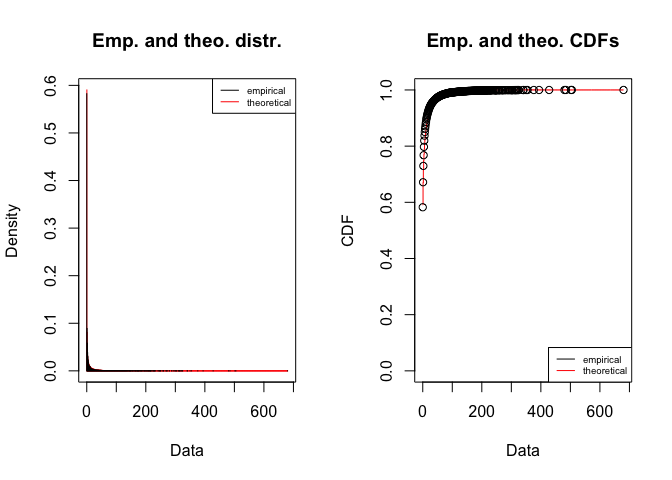
\includegraphics{dung_beetle_rarefaction_files/figure-latex/unnamed-chunk-6-1.pdf}

\hypertarget{standarize-to-number-of-individuals}{%
\subsection{Standarize to Number of
Individuals}\label{standarize-to-number-of-individuals}}

Rarefy the diversities of all localities to the lowest number of
individuals in a locality - Turner's (T\_N).

\begin{Shaded}
\begin{Highlighting}[]
\NormalTok{D\_abund\_133 }\OtherTok{\textless{}{-}} \FunctionTok{iNEXT}\NormalTok{(beetle\_counts, }\AttributeTok{datatype =} \StringTok{\textquotesingle{}abundance\textquotesingle{}}\NormalTok{, }\AttributeTok{endpoint =} \DecValTok{133}\NormalTok{)}
\FunctionTok{plot}\NormalTok{ (D\_abund\_133)}
\end{Highlighting}
\end{Shaded}

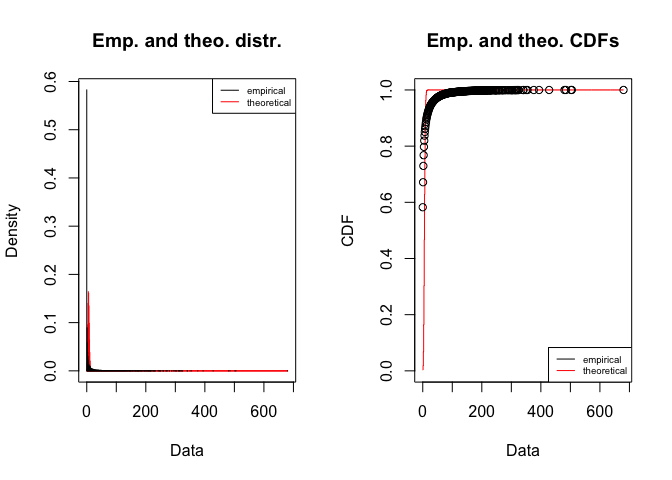
\includegraphics{dung_beetle_rarefaction_files/figure-latex/unnamed-chunk-7-1.pdf}

Calculate estimated numbers. Column qD contains the estimated diversity
for individual localities.

Orders:

\begin{itemize}
\tightlist
\item
  q = 0 for species richness\\
\item
  q = 1 for Shannon diversity\\
\item
  q = 2 for Simpson diversity
\end{itemize}

\begin{Shaded}
\begin{Highlighting}[]
\NormalTok{est\_D\_abund }\OtherTok{\textless{}{-}} \FunctionTok{estimateD}\NormalTok{ (beetle\_counts, }\AttributeTok{datatype =} \StringTok{\textquotesingle{}abundance\textquotesingle{}}\NormalTok{)}
\FunctionTok{head}\NormalTok{(est\_D\_abund)}
\end{Highlighting}
\end{Shaded}

\begin{verbatim}
##   Assemblage   m      Method Order.q        SC        qD    qD.LCL    qD.UCL
## 1        C_N 266 Rarefaction       0 0.9961664 11.973772 10.785459 13.162086
## 2        C_N 266 Rarefaction       1 0.9961664  4.992129  4.231420  5.752839
## 3        C_N 266 Rarefaction       2 0.9961664  3.436082  2.953141  3.919022
## 4       EF_N 266 Rarefaction       0 0.9946713  8.296427  7.321498  9.271357
## 5       EF_N 266 Rarefaction       1 0.9946713  3.322969  2.991965  3.653973
## 6       EF_N 266 Rarefaction       2 0.9946713  2.239294  1.996029  2.482559
\end{verbatim}

Filter out species richness.

\begin{Shaded}
\begin{Highlighting}[]
\NormalTok{D\_individuals }\OtherTok{\textless{}{-}}\NormalTok{ D\_individuals }\OtherTok{\textless{}{-}}\NormalTok{ est\_D\_abund}\SpecialCharTok{$}\NormalTok{qD[est\_D\_abund}\SpecialCharTok{$}\NormalTok{Order.q }\SpecialCharTok{==} \DecValTok{0}\NormalTok{]}
  
\CommentTok{\# filter(est\_D\_abund, Order.q == 0)}

\CommentTok{\#D\_individuals \%\textgreater{}\%}
\CommentTok{\#  select(c(Assemblage, qD))}
\end{Highlighting}
\end{Shaded}

\hypertarget{standardize-to-sample-coverage}{%
\subsection{Standardize to Sample
Coverage}\label{standardize-to-sample-coverage}}

Plot the coverage rarefaction curve for each locality. Then plot the
high end of the sample coverages.

Locality with the lowest coverage is Turner, which also had the lowest
number of individuals.

\begin{Shaded}
\begin{Highlighting}[]
\FunctionTok{plot}\NormalTok{(D\_abund, }\AttributeTok{type =} \DecValTok{3}\NormalTok{)}
\end{Highlighting}
\end{Shaded}

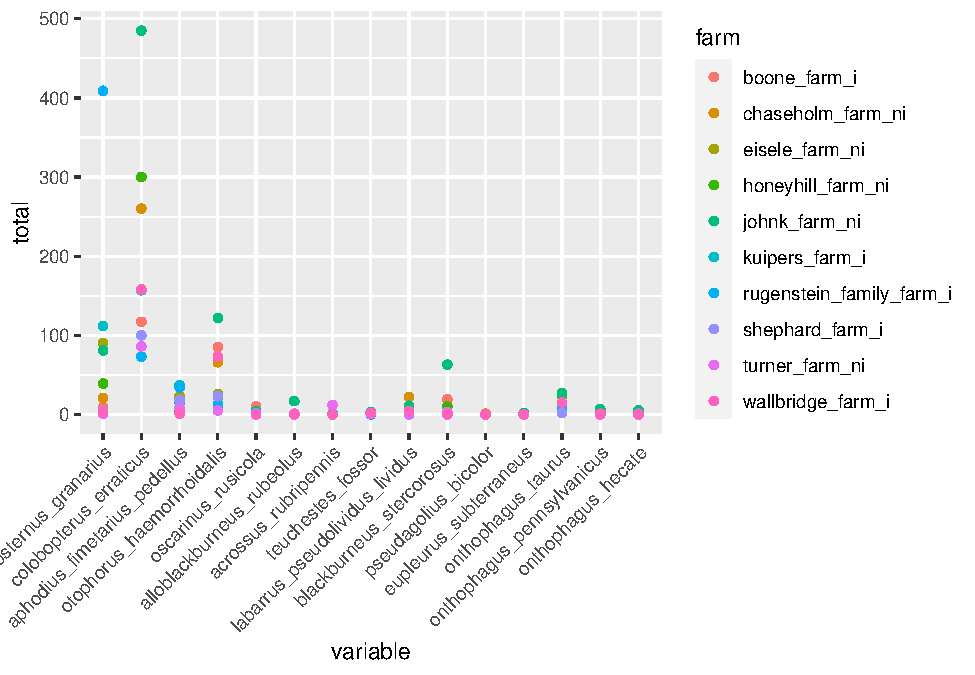
\includegraphics{dung_beetle_rarefaction_files/figure-latex/unnamed-chunk-10-1.pdf}

\begin{Shaded}
\begin{Highlighting}[]
\FunctionTok{plot}\NormalTok{ (D\_abund, }\AttributeTok{type =} \DecValTok{3}\NormalTok{, }\AttributeTok{xlim =} \FunctionTok{c}\NormalTok{(.}\DecValTok{95}\NormalTok{, }\DecValTok{1}\NormalTok{))}
\end{Highlighting}
\end{Shaded}

\includegraphics{dung_beetle_rarefaction_files/figure-latex/unnamed-chunk-10-2.pdf}

Standardize the diversities to the lowest coverage, 0.984688. Filter
again by species richness.

\begin{Shaded}
\begin{Highlighting}[]
\NormalTok{est\_D\_abund\_coverage }\OtherTok{\textless{}{-}} \FunctionTok{estimateD}\NormalTok{(beetle\_counts, }\AttributeTok{datatype =} \StringTok{\textquotesingle{}abundance\textquotesingle{}}\NormalTok{, }\AttributeTok{base =} \StringTok{\textquotesingle{}coverage\textquotesingle{}}\NormalTok{)}
\NormalTok{est\_D\_abund\_coverage}
\end{Highlighting}
\end{Shaded}

\begin{verbatim}
##    Assemblage         m        Method Order.q       SC        qD   qD.LCL
## 1         C_N 128.75935   Rarefaction       0 0.984688 10.864853 9.211780
## 2         C_N 128.75935   Rarefaction       1 0.984688  4.865750 4.117887
## 3         C_N 128.75935   Rarefaction       2 0.984688  3.402740 2.925328
## 4        EF_N  81.23609   Rarefaction       0 0.984688  6.808149 5.964588
## 5        EF_N  81.23609   Rarefaction       1 0.984688  3.210651 2.879609
## 6        EF_N  81.23609   Rarefaction       2 0.984688  2.215725 1.996672
## 7         H_N  43.01997   Rarefaction       0 0.984688  5.191303 4.647380
## 8         H_N  43.01997   Rarefaction       1 0.984688  3.739483 3.414347
## 9         H_N  43.01997   Rarefaction       2 0.984688  3.164505 2.877109
## 10       JF_N  74.73433   Rarefaction       0 0.984688  5.798019 4.988439
## 11       JF_N  74.73433   Rarefaction       1 0.984688  2.450134 2.138161
## 12       JF_N  74.73433   Rarefaction       2 0.984688  1.713307 1.526235
## 13        T_N 156.75087   Rarefaction       0 0.984688 10.591252 9.633748
## 14        T_N 156.75087   Rarefaction       1 0.984688  4.178890 3.824037
## 15        T_N 156.75087   Rarefaction       2 0.984688  2.681115 2.428028
## 16        K_I  65.21383   Rarefaction       0 0.984688  5.444569 4.411626
## 17        K_I  65.21383   Rarefaction       1 0.984688  3.371125 3.070660
## 18        K_I  65.21383   Rarefaction       2 0.984688  2.789942 2.570500
## 19       RF_I  61.80020   Rarefaction       0 0.984688  4.356026 3.932050
## 20       RF_I  61.80020   Rarefaction       1 0.984688  2.122588 1.942863
## 21       RF_I  61.80020   Rarefaction       2 0.984688  1.618959 1.498462
## 22       SF_I 171.53971 Extrapolation       0 0.984688 10.303581 5.858125
## 23       SF_I 171.53971 Extrapolation       1 0.984688  3.260604 2.593212
## 24       SF_I 171.53971 Extrapolation       2 0.984688  2.180696 1.808185
## 25        W_I 266.00000 Extrapolation       0 0.984688 12.907801 6.979502
## 26        W_I 266.00000 Extrapolation       1 0.984688  3.683673 2.893275
## 27        W_I 266.00000 Extrapolation       2 0.984688  2.259191 1.806087
## 28       BF_I 138.26982   Rarefaction       0 0.984688  6.721984 4.252357
## 29       BF_I 138.26982   Rarefaction       1 0.984688  2.732956 2.400172
## 30       BF_I 138.26982   Rarefaction       2 0.984688  2.153673 1.937373
##       qD.UCL
## 1  12.517925
## 2   5.613614
## 3   3.880152
## 4   7.651711
## 5   3.541694
## 6   2.434779
## 7   5.735225
## 8   4.064618
## 9   3.451900
## 10  6.607598
## 11  2.762106
## 12  1.900378
## 13 11.548756
## 14  4.533744
## 15  2.934201
## 16  6.477513
## 17  3.671590
## 18  3.009385
## 19  4.780003
## 20  2.302314
## 21  1.739456
## 22 14.749036
## 23  3.927996
## 24  2.553208
## 25 18.836101
## 26  4.474071
## 27  2.712295
## 28  9.191611
## 29  3.065741
## 30  2.369973
\end{verbatim}

\begin{Shaded}
\begin{Highlighting}[]
\NormalTok{D\_coverage }\OtherTok{\textless{}{-}}\NormalTok{ est\_D\_abund\_coverage}\SpecialCharTok{$}\NormalTok{qD[est\_D\_abund\_coverage}\SpecialCharTok{$}\NormalTok{Order.q }\SpecialCharTok{==} \DecValTok{0}\NormalTok{]}
  
\CommentTok{\#filter(est\_D\_abund\_coverage, Order.q == 0)}

\CommentTok{\#D\_coverage \%\textgreater{}\%}
\CommentTok{\#  select(c(Assemblage, qD))}
\end{Highlighting}
\end{Shaded}

\begin{Shaded}
\begin{Highlighting}[]
\CommentTok{\# number of observed species at each locality}
\NormalTok{D\_area }\OtherTok{\textless{}{-}} \FunctionTok{DataInfo}\NormalTok{ (beetle\_counts, }\AttributeTok{datatype =} \StringTok{\textquotesingle{}abundance\textquotesingle{}}\NormalTok{)}\SpecialCharTok{$}\NormalTok{S.obs }

\CommentTok{\# add in the estimated species richness under standardization by individuals and sample coverage}
\NormalTok{D\_est }\OtherTok{\textless{}{-}} \FunctionTok{cbind}\NormalTok{ (D\_area, D\_individuals, D\_coverage)}
\FunctionTok{rownames}\NormalTok{ (D\_est) }\OtherTok{\textless{}{-}} \FunctionTok{DataInfo}\NormalTok{ (beetle\_counts, }\AttributeTok{datatype =} \StringTok{\textquotesingle{}abundance\textquotesingle{}}\NormalTok{)}\SpecialCharTok{$}\NormalTok{Assemblage}
\end{Highlighting}
\end{Shaded}

\begin{Shaded}
\begin{Highlighting}[]
\FunctionTok{barplot}\NormalTok{(D\_est, }\AttributeTok{beside =}\NormalTok{ T, }\AttributeTok{legend.text =}\NormalTok{ T, }\AttributeTok{col =} \FunctionTok{heat.colors}\NormalTok{ (}\DecValTok{7}\NormalTok{), }\AttributeTok{xlab =} \StringTok{\textquotesingle{}Sample standardisation\textquotesingle{}}\NormalTok{,}
         \AttributeTok{ylab =} \StringTok{\textquotesingle{}Species richness\textquotesingle{}}\NormalTok{, }\AttributeTok{names.arg =} \FunctionTok{c}\NormalTok{(}\StringTok{\textquotesingle{}sample area\textquotesingle{}}\NormalTok{, }\StringTok{\textquotesingle{}\# of individuals\textquotesingle{}}\NormalTok{, }\StringTok{\textquotesingle{}sample coverage\textquotesingle{}}\NormalTok{))}
\end{Highlighting}
\end{Shaded}

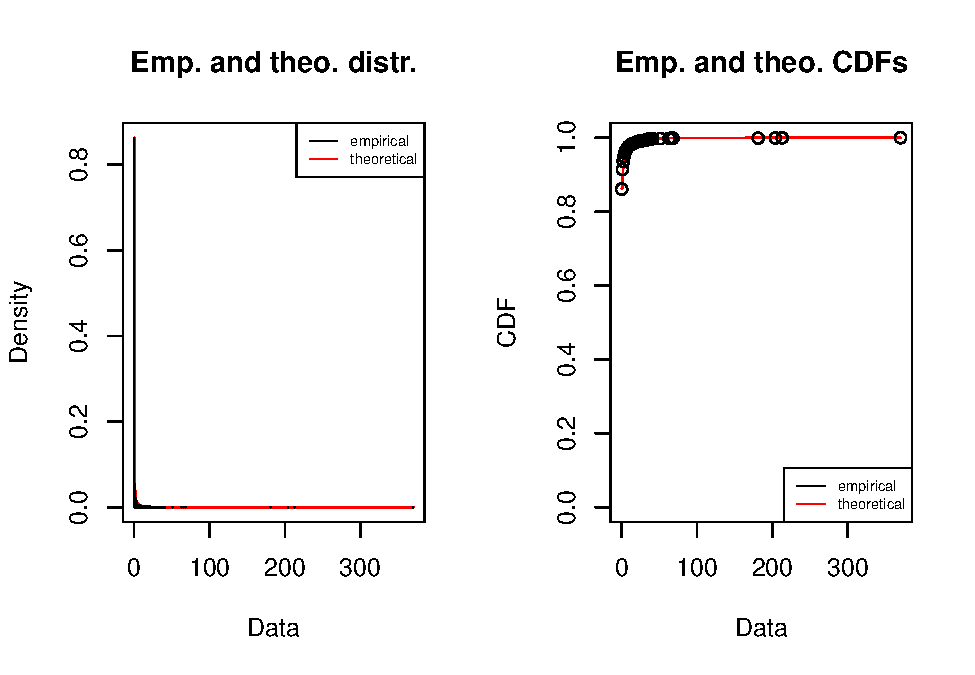
\includegraphics{dung_beetle_rarefaction_files/figure-latex/unnamed-chunk-13-1.pdf}

\begin{Shaded}
\begin{Highlighting}[]
\FunctionTok{matplot}\NormalTok{(}\FunctionTok{scale}\NormalTok{ (D\_est), }\AttributeTok{type =} \StringTok{\textquotesingle{}b\textquotesingle{}}\NormalTok{, }\AttributeTok{axes =}\NormalTok{ F, }\AttributeTok{xlab =} \StringTok{\textquotesingle{}Locality\textquotesingle{}}\NormalTok{, }\AttributeTok{ylab =} \StringTok{\textquotesingle{}Standardized species richness\textquotesingle{}}\NormalTok{)}
\FunctionTok{axis}\NormalTok{(}\DecValTok{1}\NormalTok{, }\AttributeTok{at =} \DecValTok{1}\SpecialCharTok{:}\DecValTok{10}\NormalTok{, }\AttributeTok{labels =} \FunctionTok{rownames}\NormalTok{(D\_est), }\AttributeTok{las=}\DecValTok{2}\NormalTok{)}
\FunctionTok{axis}\NormalTok{(}\DecValTok{2}\NormalTok{)}
\FunctionTok{box}\NormalTok{()}
\FunctionTok{legend}\NormalTok{(}\StringTok{\textquotesingle{}topright\textquotesingle{}}\NormalTok{, }\AttributeTok{title =} \StringTok{\textquotesingle{}Diversity standardised by:\textquotesingle{}}\NormalTok{, }\AttributeTok{legend =} \FunctionTok{c}\NormalTok{(}\StringTok{\textquotesingle{}sample area\textquotesingle{}}\NormalTok{, }\StringTok{\textquotesingle{}\# individuals\textquotesingle{}}\NormalTok{, }\StringTok{\textquotesingle{}sample coverage\textquotesingle{}}\NormalTok{), }\AttributeTok{pch =} \FunctionTok{as.character}\NormalTok{(}\DecValTok{1}\SpecialCharTok{:}\DecValTok{3}\NormalTok{), }\AttributeTok{col =} \DecValTok{1}\SpecialCharTok{:}\DecValTok{3}\NormalTok{, }\AttributeTok{lty =} \DecValTok{1}\SpecialCharTok{:}\DecValTok{3}\NormalTok{)}
\end{Highlighting}
\end{Shaded}

\includegraphics{dung_beetle_rarefaction_files/figure-latex/unnamed-chunk-14-1.pdf}

\end{document}
